\chapter{Investigating results on the limiting distribution}
\section{Playing with the (original) sequence of maxima}
\paragraph{}
Here, we will generate finite size sequences (N = 10000) of independent identically distributed random variables following respectively :
\begin{itemize}
	\item a standard Normal Distribution $\mathcal{N}(0,1)$
	\item a Cauchy Distribution \textit{Cauchy(0,1)}
	\item an Exponential Distribution \textit{Exp(1)}
\end{itemize}
We will compute the sequence of maxima, neither centred nor normalised, and draw the scatter plot as well as the plot of the maxima  $M_n$ as a function of the time steps $n$.
We will also draw the $\frac{1}{n}$-quantiles of the distributions (distributions of the sample, not of the maxima) as a function of the time steps $n$. This will lead us to make an interesting observation.
\subsection{Sample following a Normal distribution}
\paragraph{Computing the quantiles}
The Normal distribution is a particular case because, unlike in the cases of the Cauchy and the Exponential distribution, there is no explicit form to the cumulative distribution function. We will thus use a "well-known"\footnote{Many textbooks mention it, though it is not necessarily what springs to the mind when thinking about the properties of Gaussian RVs.} inequality, holding $\forall t > 0$ :
\begin{equation}
(\frac{1}{t} - \frac{1}{t^3} )*\frac{\exp(-\frac{t^2}{2})}{\sqrt{2*\pi}} < 1 - \Phi(t) < \frac{1}{t}*\frac{\exp(-\frac{t^2}{2})}{\sqrt{2*\pi}}
\end{equation}
From there, it is easy to see that the following holds :
\begin{equation}
1 - \Phi(t) \sim_{t \rightarrow +\infty} \frac{1}{t}*\frac{\exp(-\frac{t^2}{2})}{\sqrt{2*\pi}} \\
\end{equation}
When $n$ grows large, the $\frac{1}{n}$-quantile grows very large so it is valid to replace $1 - \Phi(t) $ by its equivalent in the equation satisfied by the quantiles : \\
\begin{equation}
\begin{alignat*}{2}
&\textcolor{white}{\iff} & F_X(q_\frac{1}{n}) &= 1 - \frac{1}{n} \\ 
&\iff &  \frac{1}{q_\frac{1}{n}}*\frac{\exp(-\frac{q_\frac{1}{n}^2}{2})}{\sqrt{2*\pi}}  &= \frac{1}{n} \\
&\iff & \log(q_\frac{1}{n}) + \log(\exp(-\frac{q_\frac{1}{n}^2}{2})) + \log(\sqrt{2*\pi}) &= \log(n)\\
\end{alignat*}
\end{equation}
This equation cannot be solved analytically, we will resolve it iteratively. Th starting point is $\log(n) = \frac{t_0^2}{2}$, which gives us $t_0 = \sqrt{(2*\log(n))}$. If we then run the Newton-Raphson algorithm, we see that the corrections to $t_0$ from the next iterations are small enough that we can keep $t_0$ as solution.\footnote{See the fourth of the figures below}.
\begin{figure}[h!]
	\centering
	\caption{Below, a realisation of the sequence of maxima for i.i.d. standard unit Gaussian RVs}\label{fig:toyingLimitGaussian}
\end{figure}
\begin{figure}[h!]
	\centering
	\begin{minipage}[b]{0.4\textwidth}
        \centering
        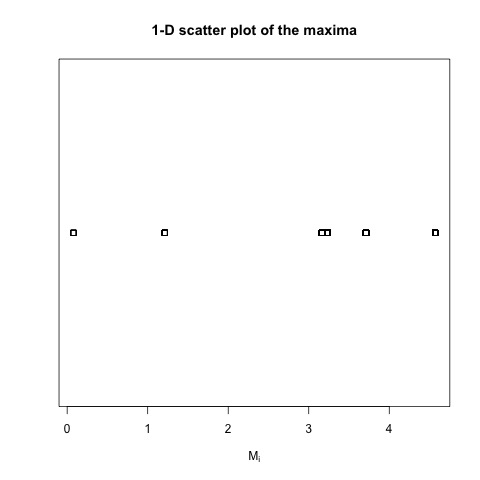
\includegraphics[scale =0.4]{/Users/kimartin/Desktop/PDM_thesis_report/latex_template5_57/main/R_Files_1/gaussianScatterMaxima.jpeg}
        \caption{Scatter Plot of the \\Maxima, n = 10000}
        \label{fig:toyingLimitGaussianScatter}
	\end{minipage}
	\begin{minipage}[b]{0.4\textwidth}
		        \centering
		        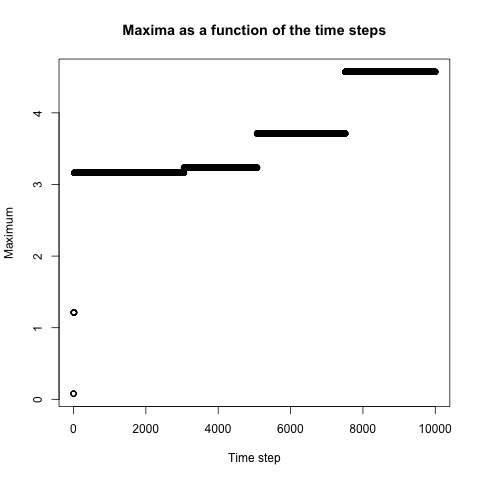
\includegraphics[scale = 0.4]{/Users/kimartin/Desktop/PDM_thesis_report/latex_template5_57/main/R_Files_1/gaussianMaximaAgainstSteps.jpeg}
		        \caption{Maxima against the time steps}
		        \label{fig:toyingLimitGaussianAgainst}
	\end{minipage}
 \end{figure}
 \begin{figure}[h!]
       \centering
       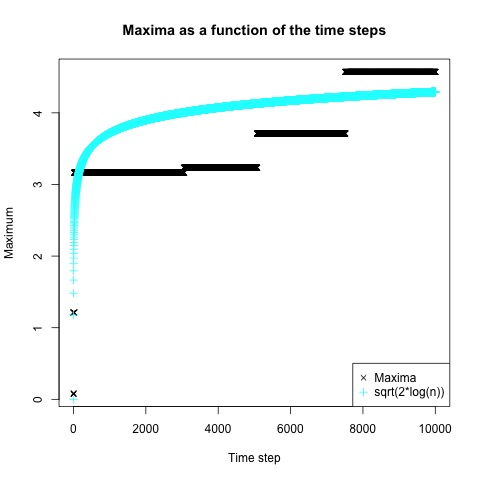
\includegraphics[scale = 0.4]{/Users/kimartin/Desktop/PDM_thesis_report/latex_template5_57/main/R_Files_1/gaussianFitting.jpeg}
       \caption{Maxima against the time steps and function n$\rightarrow \sqrt{2*\log(n)}$}
       \label{fig:toyingLimitGaussianFitting}
\end{figure}
 \begin{figure}[h!]
 	\centering
 	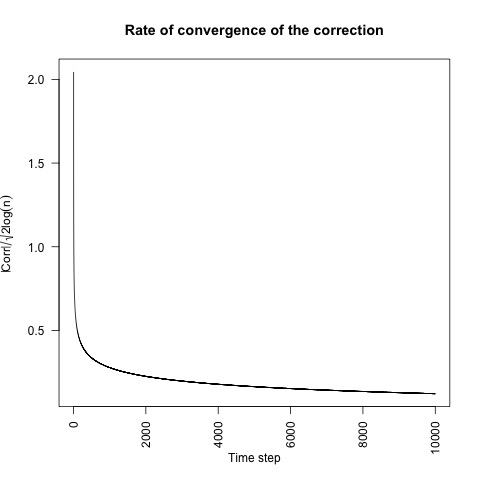
\includegraphics[scale = 0.4]{/Users/kimartin/Desktop/PDM_thesis_report/latex_template5_57/main/R_Files_3/corrApproxQuantileGaussian.jpeg}
 	\caption{The correction becomes negligible compared to the starting term as n grows large}
 	\label{fig:toyingLimitGaussianCorr}
 \end{figure}
\subsection{Sample following a Cauchy distribution}
\paragraph{Computing the quantiles}
\newline
Let $X_1, \cdots, X_n $ be i.i.d. RVs $\sim$ \textit{Cauchy(0,1)}. The distribution function is $F_X(t) = \frac{1}{\pi}*\arctan(x) - \frac{1}{2}$. The $\frac{1}{n}$-quantiles satisfy the equation : 
\newline
\begin{equation}
\begin{alignat*}{2}
&\textcolor{white}{\iff} & F_X(q_\frac{1}{n}) &= 1 - \frac{1}{n} \\ 
&\iff &  \frac{\arctan(q_\frac{1}{n})}{\pi} + \frac{1}{2} &= 1 - \frac{1}{n} \\
&\iff & \frac{\arctan(q_\frac{1}{n})}{\pi} &= \frac{2-n}{n} \\
&\iff & q_\frac{1}{n} &= \tan(\frac{\pi}{2}*\frac{2-n}{n})
\end{alignat*}
\end{equation}
\begin{figure}[h!]
		\caption{Below, a realisation of the sequence of maxima for i.i.d. \textit{Cauchy(0,1)} RVs}\label{fig:toyingLimitCauchy}
\end{figure}
\begin{figure}[h!]
	\centering
	\begin{minipage}[b]{0.4\textwidth}
		\centering
		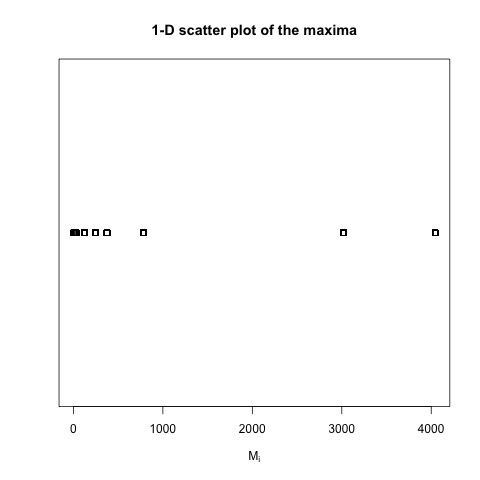
\includegraphics[scale =0.4]{/Users/kimartin/Desktop/PDM_thesis_report/latex_template5_57/main/R_Files_1/cauchyScatterMaxima.jpeg}
		\caption{Scatter Plot of the \\Maxima, n = 10000}
		\label{fig:toyingLimitCauchyScatter}
	\end{minipage}
	\begin{minipage}[b]{0.4\textwidth}
		\centering
		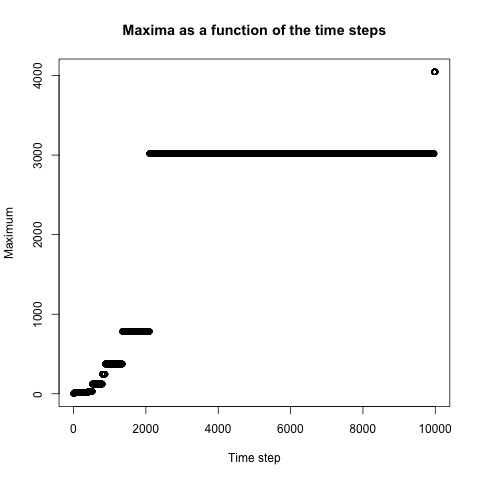
\includegraphics[scale = 0.4]{/Users/kimartin/Desktop/PDM_thesis_report/latex_template5_57/main/R_Files_1/cauchyMaximaAgainstSteps.jpeg}
		\caption{Maxima against the time steps}
		\label{fig:toyingLimitCauchyAgainst}
	\end{minipage}
\end{figure}
 \begin{figure}[h!]
 	\centering
 	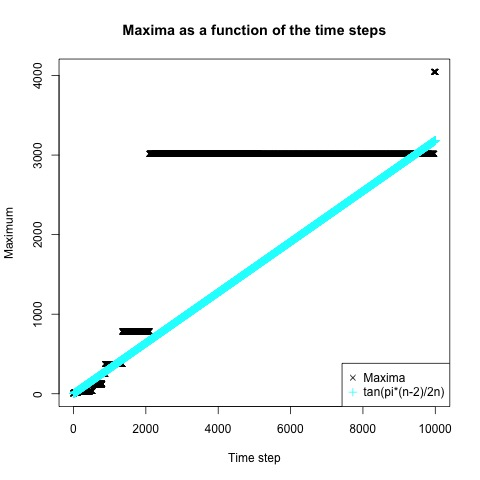
\includegraphics[scale = 0.4]{/Users/kimartin/Desktop/PDM_thesis_report/latex_template5_57/main/R_Files_1/cauchyFitting.jpeg}
    \caption{Maxima against the time steps and function n$\rightarrow \tan(pi*\frac{2-n}{2*n})}$}
    \label{fig:toyingLimitCauchyFitting}
 \end{figure}
\newpage
\subsection{Sample following an Exponential Distribution}
\paragraph{Computing the quantiles}
\newline
Let $X_1, \cdots, X_n $ be i.i.d. RVs $\sim$ \textit{Exponential($\lambda$)}. The distribution function is $F_X(t) = 1 - \exp(-\lambda*t)$. The $\frac{1}{n}$-quantiles satisfy the equation : 
\newline
\begin{equation}
\begin{alignat*}{2}
&\textcolor{white}{\iff} & F_X(q_\frac{1}{n}) &= 1 - \frac{1}{n} \\ 
&\iff & 1 - \exp(-\lambda*q_\frac{1}{n}) &= 1 - \frac{1}{n} \\
&\iff & q_\frac{1}{n} &= \frac{1}{\lambda}*\log(n)
\end{alignat*}
\end{equation}
\begin{figure}[h!]
		\caption{Below, a realisation of the sequence of maxima for i.i.d. \textit{Exp(1)} RVs}\label{fig:toyingLimitExponential}
\end{figure}
\begin{figure}[h!]
	\centering
	\begin{minipage}[b]{0.4\textwidth}
		\centering
		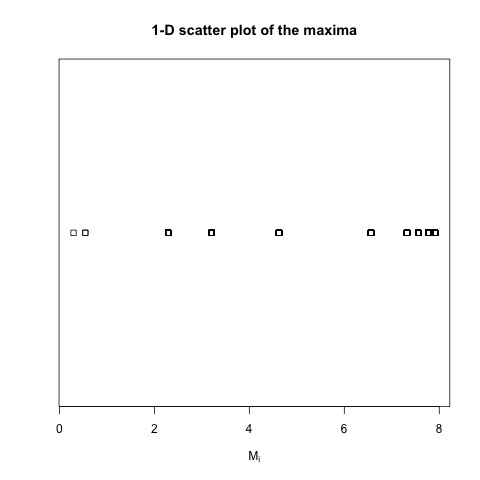
\includegraphics[scale =0.4]{/Users/kimartin/Desktop/PDM_thesis_report/latex_template5_57/main/R_Files_1/exponentialScatterMaxima.jpeg}
		\caption{Scatter Plot of the Maxima, n = 10000}
		\label{fig:toyingLimitExponentialScatter}
	\end{minipage}
	\begin{minipage}[b]{0.4\textwidth}
		\centering
		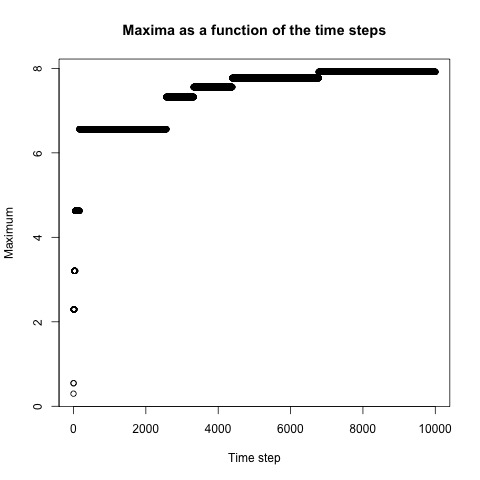
\includegraphics[scale = 0.4]{/Users/kimartin/Desktop/PDM_thesis_report/latex_template5_57/main/R_Files_1/exponentialMaximaAgainstSteps.jpeg}
		\caption{Maxima against the time steps}
		\label{fig:toyingLimitExponentialAgainst}
	\end{minipage}
\end{figure}
\begin{figure}[h!]
		\centering
		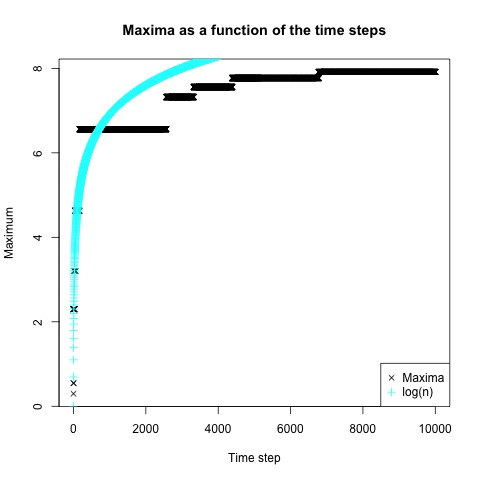
\includegraphics[scale = 0.4]{/Users/kimartin/Desktop/PDM_thesis_report/latex_template5_57/main/R_Files_1/exponentialFitting.jpeg}
		\caption{Maxima against the time steps and function n$\rightarrow \log(n)}$}
	\label{fig:toyingLimitExponentialFitting}
\end{figure}
\newpage
\subsection{Why does this work ?}

